First, our system transforms the input binary into structured
semantics we can work with throughout the rest of the process.
Second, we perform alias analysis over the structured representation.
This allows us to know all the pointers which may point to freed
memory after each free.  Finally, we look for reads and writes through
potentially freed pointers to create our list of candidate
use-after-frees.

\subsection{Alias Analysis}
Alias analysis consists of computing the possible ways to access different variables.
If dereferencing two expressions may access the same variable, they are said to alias.

Our machine-level alias analysis involves three main design choices that must be addressed:
\begin{enumerate}
\item Selecting variables.
  Alias analysis is performed over program variables, but unlike C, the assembly from a binary does not contain variable information.
\item Selecting sensitivity.
  We can return points-to information parameterized on different pieces of context.
  Common examples of parameters are flow sensitivity (program location), context sensitivity (call stack), field sensitivity (offsets within memory regions), and object sensitivity (possible construction sites for a ``this'' pointer).
  In this work, we examine, flow, context, field, and recency~\cite{vsa}, how to implement them on binary code, and their effects on precision and performance.
\item Solving for points-to relationships.
  The generation of the aliasing information is undertaken differently for flow-insensitive vs flow-sensitive varieties.
  The flow-insensitive variety uses a constraint satisfaction technique and simultaneous solving via Steensgaard~\cite{steensgaard-alias}.
  Flow-sensitive varieties use the inter-procedural dataflow described in \S \ref{sec:interproc}.
\end{enumerate}

\begin{figure}
	\centering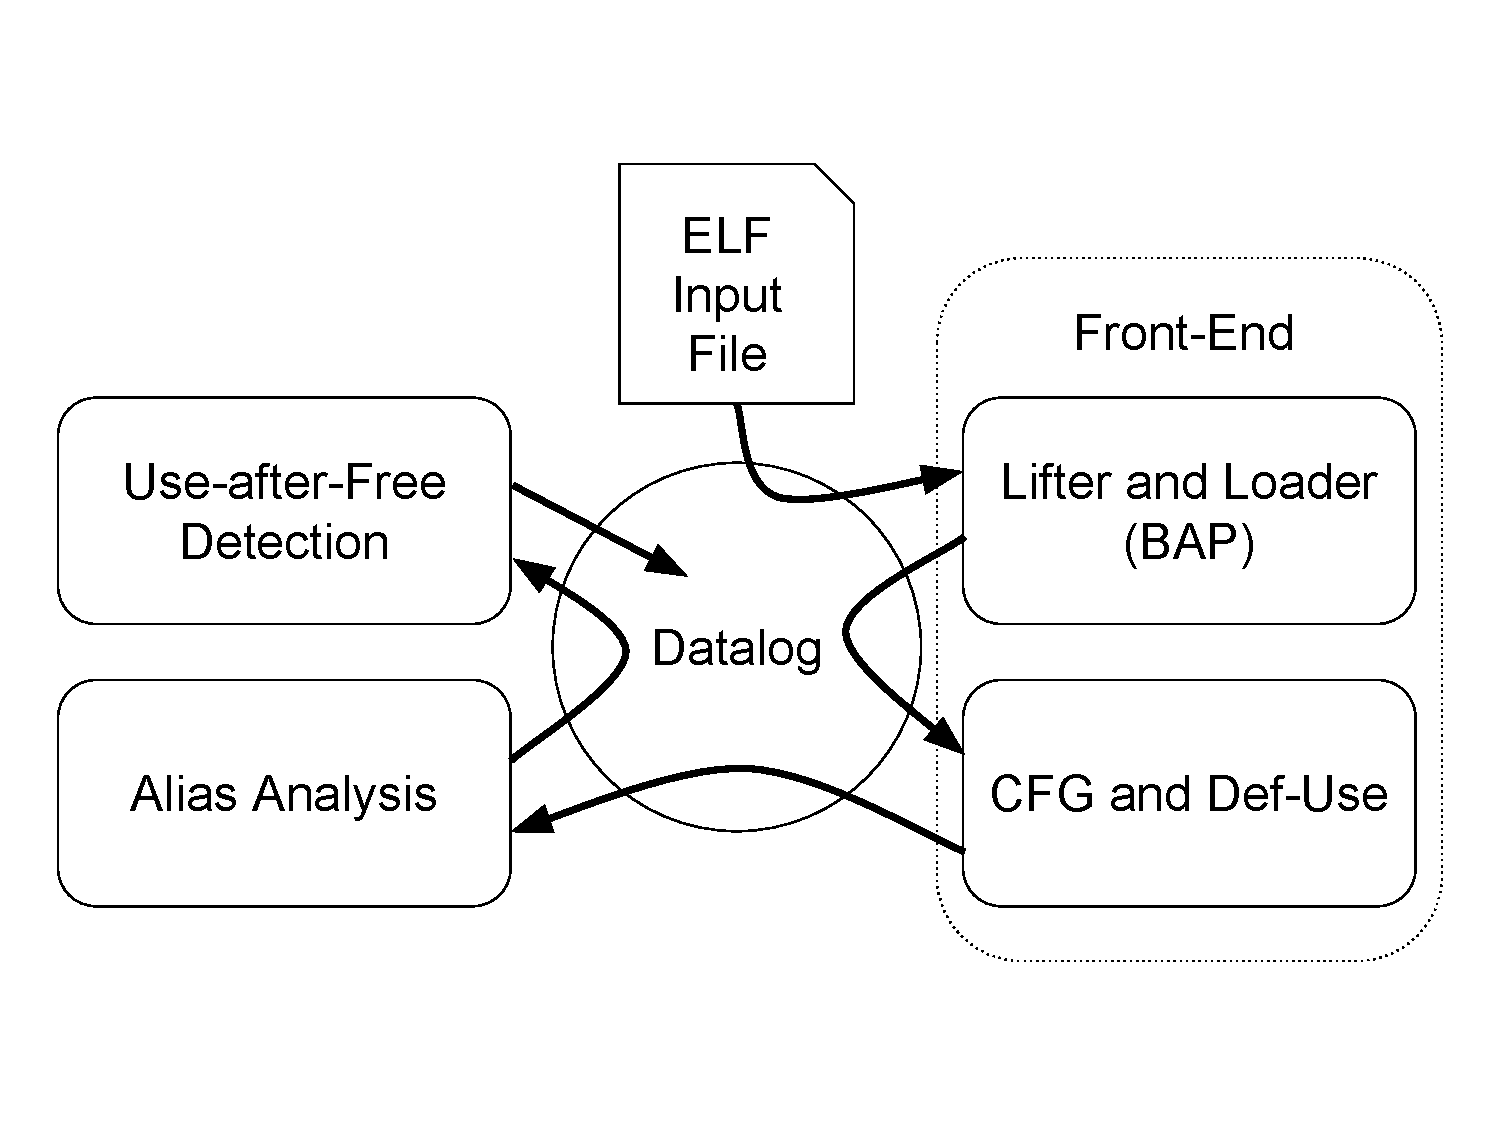
\includegraphics[scale=0.3]{alias/system.pdf}
	\caption{System Diagram}
	\label{fig:system}
\end{figure}

\subsection{Front-End}
Before we can apply our analysis, we first need to transform the raw
bytes of the input file into a form similar to the AST received after
parsing.  Techniques in this section are not novel, and are described
for completeness to understand our overall system.

The front end:
\begin{itemize}
  \item Parses the executable file container, e.g., ELF on Linux
  \item Finds potential function entry points
%TODO if I do a codependence trial, forward reference here
  \item Builds a control flow graph
  \item Provides an intermediate language with the semantics for every reachable instruction
  \item Builds a call graph and call-site information
\end{itemize}

We use the BAP~\cite{bap} framework to provide ELF parsing, entry point identification, and instruction semantics.

\subheading{Variables}
In our approach, we use 3 kinds of variables:
\begin{itemize}
	\item Stack slots, parameterized by which function they are in. Written \texttt{sp+off@func}
	\item Registers
	\item Dynamic Allocations, parameterized by the location at which they are allocated. Written \texttt{dyn@loc}
\end{itemize}
We use an abstract location in these parameterizations.
In the context-insensitive case is simply the address of the instruction, and in the context-sensitive case is the pair of the address with the return stack.

Our choice of dynamic allocation variables defines our heap model.
We assume that at two memory regions may only alias if they were allocated at the same program point.
This assumption matches reality unless a pointer has been released back to the allocator via free, but then used afterwards (a use-after-free bug).
This may violate the assumption because a write to or read from the now freed pointer may alias with newly returned memory.
As a result, this heap model is correct at least until the first use-after-free in an execution.
As we are not performing a value analysis, we also assume all accesses are in-bounds.
Essentially, if a use-after-free is the \emph{first} memory violation to occur, we will locate it.

\subheading{Calculating Update Summaries}
In order to avoid analyzing the full complexity of IL instructions within alias analysis, we first transform them to contain only the relevant dataflow information.
Our update summaries are then a description of the action of an IL instruction on the points-to relationship, where \texttt{a} and \texttt{b} are variables as defined above:

\begin{itemize}
\item \texttt{a = b}
\item \texttt{a = *b}
\item \texttt{a = \&b}
\item \texttt{*a = b}
\item \texttt{*a = *b}
\item \texttt{*a = \&b}
\end{itemize}

A list of these is generated for each instruction and associated with
the location of the instruction.  At allocation sites we emit the
summary \texttt{a = \&dyn@loc}, meaning that the variable \texttt{a}
(usually \texttt{RAX}) takes on the address of the allocation region
corresponding to that location.  % In our example~\ref{lst:example-asm}
% we would emit \texttt{RAX = \&dyn@0} for the instruction on line 4
% (location 0).  In the context-insensitive case, this gives us an
% abstraction parameterized only on the address of the malloc; values
% from one allocation site are assumed to never alias with those from
% another.  In the context-sensitive cases, this summary additionally
% parameterizes the abstraction by the return stack at allocation time.

\subsection{Insensitive Analysis}
In the flow-insensitive case, we modify the summaries before use to adapt our variable selection to better fit the problem.
Specifically, we annotate registers with definition sites, similar to what might be found in SSA form.

We compute the possible definition sites of each register on the right side of a summary, and clone the summary for every possible definition.
If the left side of a summary contains a register, we parameterize it with the location it came from.
We do this because a single register may hold many different logical variables at different points of time.
The register location parameterization allows us to avoid every definition of a register being potentially readable from every other site in the program.
Without our approach, the resulting alias sets would be too imprecise to be useful as a register's alias set (e.g., \texttt{RAX}) would include information about all variables ever assigned to \texttt{RAX} by register allocation.
Notably, this would include every call to \texttt{malloc}.
This parameterization adds a little bit of flow sensitivity even in otherwise insensitive analysis.

We then aggregate all update summaries from the program and solve them by equality via Steensgaard's algorithm.
Steensgaard runs  in almost linear time~\cite{steensgaard-alias} making it possible to compute over nearly any binary, though is less precise than flow-sensitive analysis, described below.
In this paper, we use insensitive analysis as a baseline to help quantify the additional precision derived by adding additional sensitivity.




\subsection{Adding Flow Sensitivity}
Our flow sensitive analysis is structured as a dataflow problem.  At each assembly instruction, we use a transfer
function based on Andersen's~\cite{andersen} inclusion-style analysis.
We use the inter-procedural dataflow adaptation described next (\S\ref{sec:interproc}).
The same rules and functions are used to handle both context-sensitive
and context-insensitive analysis, as the Location's stack context is
considered optional.

A dataflow analysis is defined by a transfer function which calculates how a statement should update the dataflow facts
(alias sets in our case),
a set of control flow edges to walk from a set of starting points,
and a meet function with specifies how to merge information sets at control flow graph confluence points.
We describe these below.

By default, alias analysis calculates alias sets even when a variable is dead.
We run a path before alias analysis to determine which variables are live.
While calculating alias analysis, we use this information to remove dead points-to information to improve performance and precision.
Performance is increased because we do not waste time and space updating and tracking points-to
sets we know will never be used.
Precision is increased because if no pointers to a given allocation exist any longer, we know any new pointer to that allocation points to copy of that region which does not need the information from the old copy.

\subheading{Transfer Function}
The actual processing of the update summaries based on summaries is
calculated via the transfer function.  We follow Andersen as shown
shown in Listing \ref{lst:process}:
\begin{itemize}
\item Definitions of variables are performed destructively.
\item Writes through variables are applied to each value they may point to.
\item Right hand sides go through 0, 1, or 2 levels of dereference for \texttt{\&b}, \texttt{b}, and \texttt{*b} respectively to generate the set to update with
\end{itemize}

\begin{figure}
	\centering
	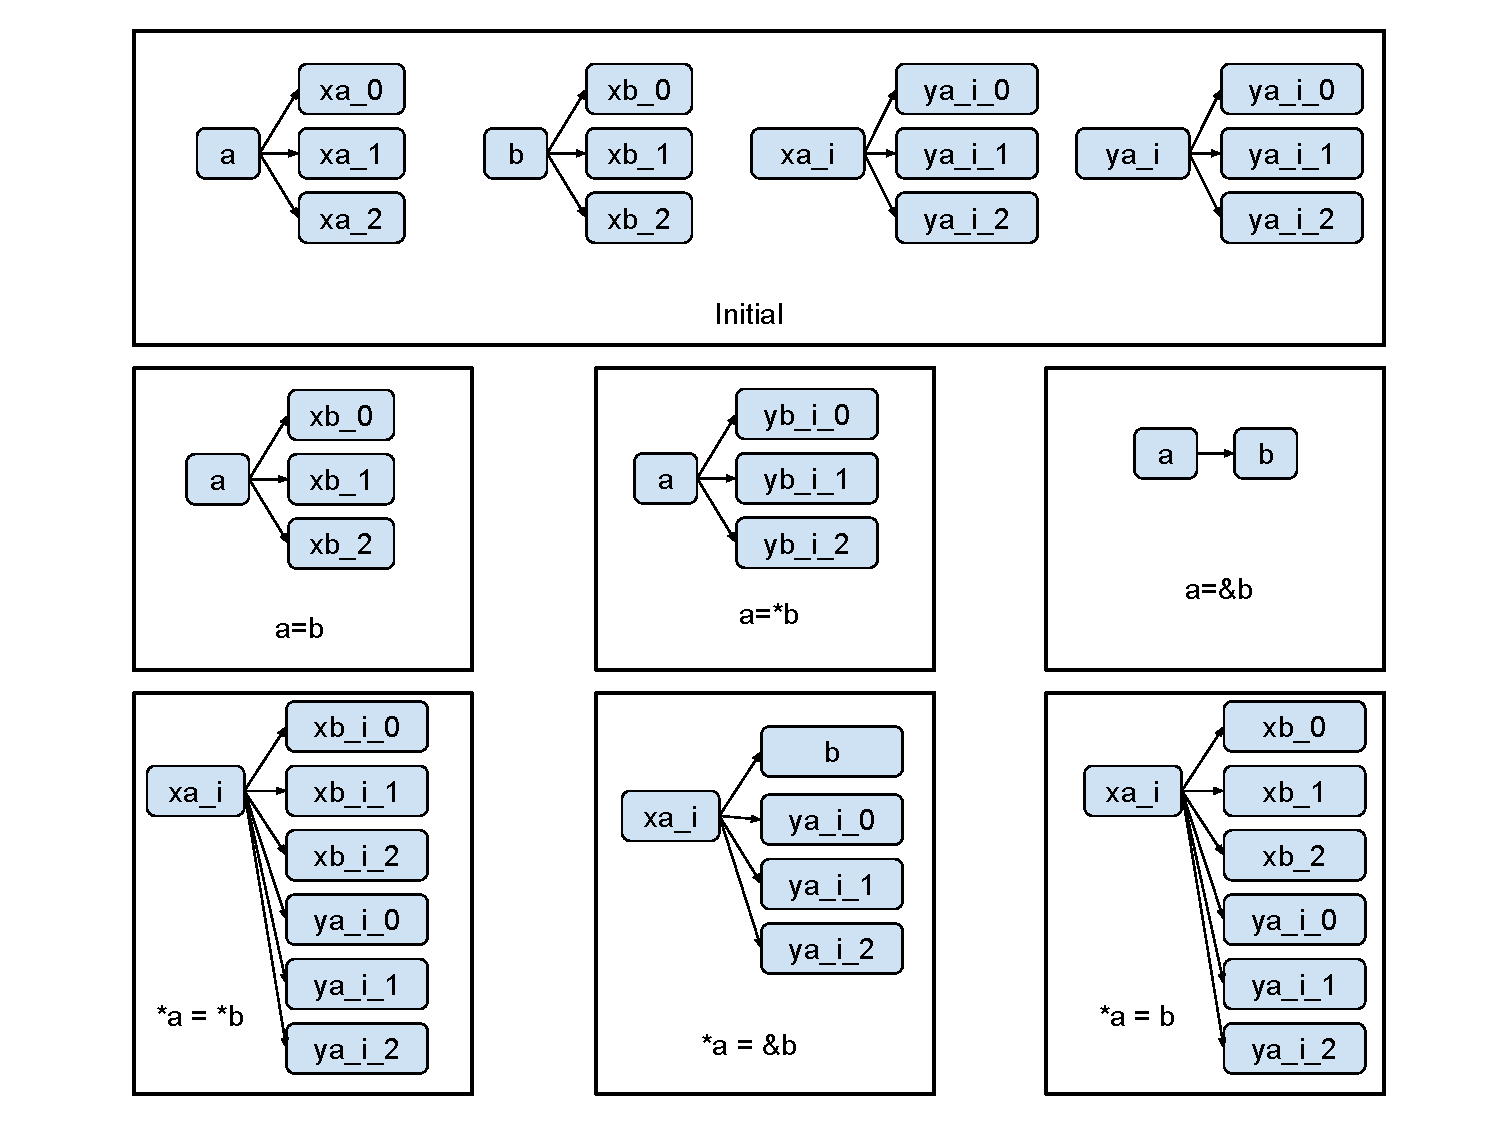
\includegraphics[scale=0.35]{alias/pts-update.pdf}
	\caption{Points-to Updates}
	\label{fig:pts-update}
\end{figure}

Figure~\ref{fig:pts-update} shows the transfer function rules for each
statement type.
%This is illustrated in Figure \ref{fig:pts-update}.
The ``Initial'' section shows a sample initial configuration a points-to relation might have.
Each other region is labeled by a statement, and shows what would change about the points-to relation.
Each time an ``i'' is used on the left, assume that portion is present 3 times, with i ranging from 0 to 2.

For updates to stack slots or registers, we can perform a ``destructive'' update.
You can see this in the \texttt{a =} examples in Figure \ref{fig:pts-update}.
This means that since we know the new value
is the only value the variable could have, we can \emph{replace} the
points-to set.  In the case of pointer write though, we cannot do
this, because our analysis is not field sensitive.

In a field sensitive analysis, this destructive update logic would be
extended to writes through pointers with a points-to size of one,
allowing for more destructive updates and increasing the precision of
our analysis.
We will explain and add field sensitivity shortly in section \ref{sec:field}, but until then, pointer updates need to remain non-destructive.

After we complete the updates to the points-to structure, we remove
all variables which are no longer live according to the previously computed information.
These variables will never be used, so tracking them is imprecise and expensive.

Finally, we perform a mark-and-sweep garbage collection of the tracked pointers, using stack slots, registers, and anything that was pointed to at the entrance of the function as roots.
This last caveat is necessary so that if an argument to a function is written to, and then never used again, the parent will still see the update even though the callee no longer knows how to reference the region.
This allows us to \emph{forget} about allocations which are no longer accessible.

\paragraph{Dataflow}
\begin{lstlisting}[float=*t, caption={Flow Sensitive Pointer Analysis Rules}, label=lst:flowrules]
flow_in(Location, PointsTo^pt_union)
flow_out(Location, PointsTo)

flow_init: flow_in(loc, {}) <- malloc_call {loc}

flow_step: flow_in(dst, pts) <-
  succ {src, dst, is_call: false, is_ret: false} & flow_out(src, pts)

flow_xfer: flow_out(loc, pts2) <-
  flow_in(loc, pts) & updates(loc, us) & kill(loc, ks) & live {loc, live}
  & flow::xfer(pts, us, ks, pts2)
\end{lstlisting}
\begin{lstlisting}[float=t, caption={Process Update}, label=lst:process]
match update {
  (*\bfseries *a = \&b*) =>
    for a_target in pts[a] {
      pts_out.add(a_target, b)
    }
   (*\bfseries a = \&b*) =>
     pts_out.replace(a, {b})
   (*\bfseries a =  b*) =>
     pts_out.replace(a, pts[b])
   (*\bfseries a = *b*) =>
     pts_out.replace(pts[pts[b]])
  (*\bfseries *a =  b*) =>
    for a_target in pts[a] {
      pts_out.add(a_target, pts[b])
    }
  (*\bfseries *a = *b*) =>
    for a_target in pts[a] {
      pts_out.add(a_target,
                  pts[pts[b]])
    }
}
\end{lstlisting}

The overall flow rules we use are shown in  Listing \ref{lst:flowrules}.
Andersen-style analysis formulates updates as inclusion constraints, rather than equality constraints like Steensgaard.
In the initial declaration of predicates, \texttt{flow\_in} is declared to aggregate via set union on each points-to set.
Since each \texttt{flow\_in} value at a location produces a unique \texttt{flow\_out} value, aggregation is not necessary on that predicate.
We create an empty input map at every allocation site, because allocation is the only action which will add information to an empty points-to relation.
\texttt{flow\_step} propagates points-to relations along normal succession edges.
Finally, \texttt{flow\_xfer} performs the meat of the operation, absorbing the update summaries into the current context by applying the transfer function.

\subsection{Inter-procedural Dataflow}
\label{sec:interproc}
Our approach to inter-procedural dataflow follows the example of Reps~\cite{interproc-dataflow} with some modifications.
While many optimizations described there are inapplicable to our domain, the general structure still applies.
At the site of a call, an inter-procedural edge is added from the call site to the target function.
Following this edge elides stack slots which are not currently pointed to.
This is a departure from Reps in that their restricted domain, all local variables were not passed through.
An intra-procedural edge is added which skips over the call, applying effects (see \S \ref{sec:effects}) and clobbering variables not preserved by the function.
Finally, at each return site, an inter-procedural edge which forgets the stack slots local to that function if not pointed to is added.
\footnote{You might wonder why we don't report an error if a local stack slot is pointed to, or why this needs to be checked for. This is a legal possibility in the case of a recursive call which passes one of its stack variables to itself by reference.}
Again, we depart from Reps here by keeping around what would normally be local variables if they are pointed to.

\texttt{flow\_call} and \texttt{flow\_ret} apply when functions are entered and exited to cut down on unnecessary information being propagated around, applying the restrictions for our inter-procedural edges, as described earlier.

\texttt{flow\_call\_over} propagates information at a call site \emph{over} a function call, skipping it but removing definitions for variables known to be overwritten by the function.
This corresponds to the special intra-procedural edge added to our dataflow when processing a call.
This rule also enables analysis through functions which were not provided, albeit with the assumption that the function was effectively a no-op.

\begin{lstlisting}[float=*t, caption={Inter-procedural Rules}, label=lst:interrules]
flow_call: flow_in(dst, pts2) <-
  succ {src, dst, is_call: true} & flow_out(src, pts)
  & flow::call(pts, dst, pts2)
flow_ret: flow_in(dst, pts2) <-
  succ {src, dst, is_ret: true} & flow_out(src, pts) & func {base, contains: dst}
  & flow::ret(pts, base, pts2)
flow_call_over: flow_in(dst, pts2) <-
  call_over {src, func, dst} & flow_out(src, pts)
  & flow::over(pts, pts2)
\end{lstlisting}

\begin{lstlisting}[language=C, float=t, caption={Example (C)}, label=lst:example-c]
char* g() {
	return malloc(1);
}
void f() {
	char* x = malloc(1);
	*x = 'a'; // Safe
	char* g_a = g();
	*g_a = 'a'; // Safe
	char* g_b = g();
	*g_b = 'a'; // Safe
	free(x);
	free(g_a);
	*x = 'b'; // UaF
	*g_b = 'b'; // Safe, but needs context
}
\end{lstlisting}

\subsection{Inter-procedural Flow-Sensitive Example}
In this section, we provide an example of the context- and flow-
sensitive analysis on a simple example shown in
Listing~\ref{lst:example-c}. To provide clarity on how updating alias
sets work, this example does not show data-flow merges, which is a set
union operation as previously described.

Listing \ref{lst:example-c} contains one real use-after-free bug.  We
also show one location that is safe, but without context-sensitivity
an additional false positive will be raised. Without
context-sensitivity, both the allocations for \texttt{g\_a} and
\texttt{g\_b} get merged, making the analysis believe they are aliased
when they are not.

\lstdefinestyle{hilight-asm}{
    language={[x86masm]Assembler},
    moredelim=[is][\color{green}]{|+}{|},
    moredelim=[is][\color{blue}]{|!}{|},
    moredelim=[is][]{|~}{|},
    basicstyle=\footnotesize 
}

\lstinputlisting[style=hilight-asm,
caption={Annotated Flow-Insensitive Analysis},
label=lst:example-asm]{alias/example-annotated.asm}

The corresponding assembly, annotated with comments on the location of
the UaF and alias sets, is shown in Listing~\ref{lst:example-asm}.
Portions of the alias set hilighted in green are new bindings.
Portions in blue are bindings which have been destructively updated.
In the example, the variables are:
\begin{itemize}
	\item The stack slots of f (g has none): sp+24@f, sp+16@f, sp+8@f
	\item All used registers (other than the stack): RDI, RAX
	\item Allocations split on sensitivity, using the form dyn@addr\{stack\}
          \begin{itemize}
          \item Context-insensitive: dyn@5 and dyn@13
          \item Context-sensitive: dyn@5\{19\}, dyn@5\{25\}, dyn@13\{\}
          \end{itemize}
\end{itemize}

The alias sets are annotated as comments. For example, right before
the free on line 35, the alias set is:

\begin{figure}[h!]
\texttt{\{ RAX -> dyn@0; sp+24@f -> dyn@1;
    sp+16@f -> dyn@0; sp+8@f -> dyn@0;
    RDI -> dyn@0 \}}
\end{figure}

This shows that \texttt{RDI} is pointing to the memory location \texttt{dyn@1}, the allocation site for \texttt{x} in the source code.
Right after the \texttt{free} on line 35, the alias set changes to show \texttt{dyn@1} is now free.
The UAF detector would say any pointer that resolves to \texttt{dyn@1} is therefore a use-after-free bug, which happens on
line 53.

If we had been context-sensitive, the points-to relation at 59, the false positive, would instead be
\begin{figure}[h!]
\texttt{\{ RAX -> dyn@5\{25\}; sp+24@f -> dyn@13\{\};
    sp+16@f -> dyn@5\{19\}; sp+8@f -> dyn@5\{25\};
    RDI -> dyn@5\{19\}; dyn@13\{\} -> free@35;
    dyn@5\{19\} -> free@43 \}}
\end{figure}

The key difference here is that \texttt{RAX} points to \texttt{dyn@5\{25\}} rather than just \texttt{dyn@5}, so we can distinguish it from the freed allocation.
This allows context sensitivity to weed out more false positives.




\subsection{Adding Context Sensitivity}
Context-sensitivity requires we only change our \texttt{Location}
values to contain information about the stack.
We add an empty stack to entry points to initialize the new stack-enhanced CFG.
Called functions must copy their control flow graphs to separate versions for every stack at which they are being called.
When generating the target of a call function, we now add the current instruction's fallthrough to the stack as a return address.
If the return address is already on the stack, we truncate the stack so that it is the topmost.

Unfortunately, with an unbounded stack, of our real-world samples, this approach exhausts available resources (128G RAM) for all but \texttt{gnome-nettool}.
To remedy this, we use a $k$-stack approach combined with the stack truncation above.
If a call is made from a location parameterized by a stack, it is first checked to see if the call site is present.
If so, it is truncated as before.
Otherwise, it is pushed onto the stack, and if the stack is longer than $k$, the oldest entry is removed.
In the case of our example, a stack size of 1 would be sufficient, and we'd see the allocations \texttt{dyn@0\{10\}}, \texttt{dyn@0\{11\}}, and \texttt{dyn@1\{\}}.

\subsection{Adding Field Sensitivity}
\label{sec:field}
%TODO add arith and widening
Up until now, we've been treating each memory region like a single homogeneous bag:
Anything written into it ever can be read out again on any subsequent read.
This reduces precision.

In traditional alias analysis, field sensitivity can be done by simply treating each variable with a struct type as though it were several - one for each field.
Unfortunately, in the binary case, things are slightly messier for two reasons: overlapping fields, and variable offset writes.
Since this is only a pointer analysis, not a general value analysis, we only consider fields with size equal to the pointer size.

Previously, we used a simple set to denote what a variable might point to.
We now replace this with a ``field map''.
We will use the word ``reference'' to describe the pair of a variable and an offset.
The offset may be a fixed value, or a special value indicating a computed offset.

A field map has two components: a set of references for unknown offsets, and a set of references for some subset of possible fixed offsets.
If a fixed offset read is performed, we return the offset's set if defined, otherwise the unknown set.
If a computed offset read is performed, we return the union of every set (both unknown and fixed) present in the map.

We split update rules into cases for a single pointer write (so we know which memory cell was updated precisely) and for multiple.

\subheading{Single Pointer}
If a fixed offset write is performed on a variable, we destructively update the set corresponding to that offset.
If a computed offset write is performed, we extend both the unknown set, and every tracked offset to contain the new reference.
If an overlapping field is written to, the field it overlaps is emptied.

\subheading{Multiple Pointers}
If a fixed offset write is performed on a variable, extend the set corresponding to that offset.
If a computed offset write is performed, we extend both the unknown set, and every tracked offset to contain the new reference.
If an overlapping field is written to, nothing happens.

This structure is conservative so long as we accept the assumption that pointers are not constructed piece-wise.
Specifically, if pointers are constructed over the course of multiple writes, we will not know about them.
This limitation was present in the previous, field insensitive formulation, but becomes more obvious in the description of the field sensitive extension.
This practice is extremely uncommon (outside bulk copy functions like \texttt{memcpy}, which may be summarized), so we accept this limitation to limit the need to reason about the exact possible values of a computed offset.

Unfortunately, this formulation gives the alias analyzer slightly too much power.
Specifically, it can now count.
Despite the fact that we did not model actually performing arithmetic, a pointer being incremented in a loop will look like repeatedly examining relative offsets of a struct.
To deal with this, we add a widening operator which, if the same variable points to a fixed limit or more offsets in a region, will replace it with pointing to an unknown offset to that region.
This reclaims termination.

\subsection{Recent Allocation Domain}
\label{sec:effects}
Using the site or site and size of an allocation to define the allocation domain is fairly common.
However, this can have poor behavior around loops:

\begin{lstlisting}
char* x;
while(1) {
site_0:
	x = malloc(1);
	*x = 'a';
	free(x);
}
\end{lstlisting}

If running a dataflow computation to fixpoint, on the second
iteration, the allocation for \texttt{site\_0} will appear already
freed.  The usual response to this type of imprecision is to unroll
loops a fixed number of times.  However, our tool is intended to be
complete (assuming a complete control flow graph, provided functions,
etc.) so we want to avoid fixed unrollings.

To this end, we extend our allocation domain with a ``recent'' bit,
similar to the MRAB/NMRAB abstraction~\cite{vsa}, though for different
purposes.  In terms of a concrete trace, the address most recently
given by an allocation at a given site belongs to the set where
``recent'' is true.  All other addresses issued by that site belong to
the set where ``recent'' is false.  In our static form, an address
belongs to the recent if there exists some trace for which it was the
last allocated from that site.  It belongs to the non-recent set if
there exists some trace for which it was not most recently allocated.
Note that once in static form, the recent set may have more than one
member, and may even intersect with the non-recent set.

This extension is a departure from the normal Andersen alias analysis.
It is only for precision, not correctness.
It can essentially be viewed as 1 bit path-sensitivity, where path-sensitivity would be parameterizing on the entire sequence of instructions taken to reach the current point.

Implementing this in our static approach means we need to make a few changes.
When an allocation summary is processed by the points-to relation, all other references to that allocation have their recent bit set to false.
We also need to modify the behavior of \texttt{flow\_call\_over} to update the caller to represent what may have happened in the callee.

We define an ``effect'' to be a set of definite allocation sites and a set of possible allocation sites that occur when a call is made.
To apply an effect to a points-to set:
For every definite allocation site, make the recent bit false.
For every possible allocation site, duplicate any recent references to
have both recent and non-recent values. Listing~\ref{lst:recent} shows
this change.

%To this end, we amend the rules as in Listing \ref{lst:recent}
\begin{lstlisting}[float=*t, caption={Rules for Recent Domain}, label=lst:recent]
flow_call_over: flow_in(dst, pts2) <-
  call_over {src, func, dst} &
  flow_out(src, pts) &
  (*\bfseries func\_effect \{func, effect\} \&*)
  (*\bfseries flow::over\_effect(pts, effect, pts2)*)

local_effect {base: Location, local: Location, effect: Effect}
func_effect {func: Location, effect: Effect^effect_merge}

effect_init: local_effect {base, local: base, effect: no_op} <- func {base}
effect_ret: local_ret: func_effect(base, effect) <-
  succ {src: local, is_ret: true} &
  local_effect {base, local, effect}
effect_xfer: local_effect {base, local: local2, effect} <-
  succ {src: local, dst: local2, is_call: false, is_ret: false} &
  local_effect {base, local, effect}
effect_call: local_effect {base, local: local2, effect: effect2} <-
  call_over {src: local, func: remote, dst: local2} &
  func_effect {func: remote, effect: effect_call} &
  local_effect {base, local, effect} &
  effect::sequence_effect(effect, effect_call, effect2)
effect_malloc: local_effect {base, local: local2, effect: effect2} <-
  succ_over {src: local, dst: local2} &
  local_effect {base, local, effect} &
  malloc_call {loc: local} &
  effect::malloc(effect, local, effect2)
\end{lstlisting}

There are four new functions here.
\texttt{effect\_merge} will merge two local effects at a confluence point.
It does this by intersecting their definite allocations, and migrating all other allocations to possible allocations.
\texttt{flow::over\_effect} will apply the effect to the points-to set in addition to its earlier responsibilities.
\texttt{effect::sequence\_effect} will update the currently processed effect with the called function's effect by unioning together both possible and definite effects, then removing those possible effects which are also definite.
\texttt{effect::malloc} just adds the current site as a definite allocation to the effect.

The result is that these effect summaries allow greater precision over allocation sites, similar to what is achieved through loop unrolling, but without sacrificing fix-point semantics.

In our example earlier, this would give rise to three allocations - \texttt{dyn@0}, \texttt{dyn@1+old}, and \texttt{dyn@1}.
This would suppress the false positive by distinguishing between the two invocations of \texttt{g}.
However, were a third added, it would not be able to distinguish between the first two invocations of \texttt{g}.

\subsection{Use-after-Free}
With alias relationship in hand, we must determine which reads and writes in the program are use-after-free candidates.
For the flow and flow \& context analyses, we can augment the alias analysis itself to track most of this information for us.
When a free occurs, we generate a special form of the \texttt{*a = \&b} summary, with \texttt{a} as the pointer being freed, and \texttt{b} as a special value representing things freed at that location.
This is as presented in Listing \ref{lst:uafflow}.
\texttt{read\_vars} generates pointer access information from actual assembly instructions, and \texttt{use\_vars} imports it from summaries which can do things like determine argument count to \texttt{printf}.

\begin{lstlisting}[label=lst:uafflow, caption={Tracking Frees with Flow Sensitivity}]
read_vars: deref_var(v, loc) <-
  lift {loc, bil} &
  func {base, contains: loc} &
  uaf::reads_vars(bil, v)
use_vars: deref_var(v, loc) <-
  uses(r, loc) &
  uaf::use_vars(r, v)

free_summary: summary(loc, s) <-
  free_call{loc, args} &
  uaf::free_summary(args, s)
uaf_flow: uaf_flow(v, loc, loc2) <-
  deref_var(v, loc2) &
  flow_in(loc2, pts) &
  flow::is_freed(pts, v, loc)
\end{lstlisting}

However, this approach only works with alias information that is at least flow sensitive.
Without flow sensitivity, any pointer which was ever freed will appear freed everywhere in the program, even before it was freed.
As a result, the false positive rate would be absurd, and such a detector would be more a heap-access detector than a use after free detector.
To help it along and make the difference in false positive rates more about the precision of the alias information rather than the ability to track state changes, we add a few extra conditions to report a use after free without flow sensitivity by essentially doing flow sensitive tracking of the freed-property only.

\begin{lstlisting}[label=lst:uafins, caption={Tracking Frees Insensitively}]
base_freed: freed_base(v, loc) <-
  free_call {loc, args} &
  uaf::free_args(args, v)
all_freed: freed_var(v2, loc) <-
  freed_base(v, loc) &
  steens_point(v, vs) &
  uaf::expand_vars(vs, v2)

path_init: path_exists(loc, loc) <-
  freed_base(_, loc)
path_step: path_exists(loc, loc3) <-
  path_exists(loc, loc2) &
  succ_any {src: loc2, dst: loc3}

uaf: uaf(v, loc, loc2) <- freed_var(v, loc) & path_exists(loc, loc2) & deref_var(v, loc2)
\end{lstlisting}

The implementation of this modification is shown in Listing \ref{lst:uafins}.
In the first stanza, we mark the variable freed by the free call and everything it aliases with as potentially freed at that location.
In the next, we find those parts of the program reachable from the free site.
We then finalize the results by saying that if a path exists from a freed variable to a dereference of that same variable, then there is a use after free candidate.
While this is certainly imperfect, going much further would begin to graft flow sensitive information into the otherwise insensitive analysis.

\subsection{Limitations}
Our system is conservative in almost all cases, but there are a few notable exceptions.
If the provided file is linked against files which are not provided, their functions will be assumed to effectively be no-ops.
If in reality, these functions free memory or write to the heap, this may cause missed vulnerabilities.
Currently, we do not resolve indirect jumps other than returns, assuming they go nowhere.
This may result in an incomplete control flow graph, which in turn can lead to missed bugs.
ssentially, if a prerequisite step gives our algorithm incomplete information, it will produce an incomplete result.
This was sufficient for the programs analyzed, which are written largely in C, but some resolution would be required to achieve good quality result on C++ programs which use vtables or programs which use a callback architecture (and so rely heavily on function pointers).

We assume the transfer of a pointer from one place to another will take place in a single assembly instruction - we do not model ``the first 3 bytes of a pointer to x'' for example.
Finally, we assume that a traditional stack discipline is being followed for purposes of points-to minimization in the sensitive cases.
If it is not, aliases from stack calculations pointing above or below your own stack frame may be missed.
